
\documentclass[12pt,a4paper,oneside]{book}
\usepackage[utf8]{inputenc}
\usepackage{amsmath}
\usepackage{amsfonts}
\usepackage{amssymb}
\usepackage[spanish]{babel}
\usepackage[graphicx]{realboxes}
\usepackage{wrapfig}
\usepackage{fancyhdr}
\usepackage[hidelinks]{hyperref}
\usepackage{datatool}
% \usepackage[acronym]{glossaries}
\usepackage{glossaries}
\usepackage{makeidx}
\usepackage{multirow}
\usepackage{multicol}
\usepackage{colortbl}
\usepackage{cite}
\usepackage{IEEEtrantools}
% \usepackage{ieeetrantools}
\usepackage{float}
\makeindex
\pagestyle{fancy}

\makeglossaries % este comando debe estar en el preámbulo

\begin{document}
% \renewcommand{\glossaryname}{Glosario}

\renewcommand\listtablename{\'Indice de Tablas}
%\listtablename

\renewcommand{\tablename}{Tabla}
\renewcommand{\acronymname}{Acronimos y simbolos}
\renewcommand{\bibname}{Referencias bibliograficas}
%\glsaddall
\frontmatter
\vspace*{-3cm}
\begin{figure}[h]
\leavevmode
\begin{minipage}{\textwidth}
\begin{center}
%\includegraphics[scale=0.5]{./logofpune}
\end{center}
\end{minipage}
\end{figure}

\thispagestyle{empty}

{\bf
\begin{center}
\large
\vspace*{-1 cm}\Large \textsc{Universidad Nacional del Este.} \\
\Large \textsc{Facultad Politécnica.} \\
\vspace*{0.5 cm}\hrule
\end{center}
}

\vspace*{-0.5 cm}
\begin{figure}[htb]
\begin{center}

\includegraphics[scale = .6]{./portada_y_ficha_catalografica/logo.png}

\end{center}
\end{figure}


\vspace{3 cm}
{
\noindent
\begin{center}
\huge \bf $<$Sistema experto para la gestión de fallas en refrigeración industrial critica$>$.
\end{center}
}


\vspace{6 cm}

\begin{center}
{\textbf{\Large $<$Teofilo Vergara Acosta$>$.}\\[5mm]
\vspace{1 cm}
\textbf{Año \the\year.}}
\end{center}

\bstctlcite{IEEEexample:BSTcontrol} % cambia "and" por "y" en bibliografía

\vspace*{-3cm}
\begin{figure}[h]
\leavevmode
\begin{minipage}{\textwidth}
\begin{center}
%\includegraphics[scale=0.5]{./logofpune}
\end{center}
\end{minipage}
\end{figure}

\thispagestyle{empty}

{\bf
\begin{center}
\large
\vspace*{-1 cm}\Large \textsc{Universidad Nacional del Este.} \\
\Large \textsc{Facultad Politécnica.} \\
\vspace*{0.5 cm}\hrule
\vspace*{0.5 cm}\Large Carrera $<$Nombre de la Carrera.\\
\vspace*{0 cm}\Large Cátedra Nombre de la Cátedra.\\
\end{center}
}

\vspace{3.5 cm}
{
\noindent
\begin{center}
\huge \bf Sistema Experto para la gestion de fallas en refrigeracion industrial critica.
\end{center}
}


\vspace{0.5 cm}
{ 

Por: \textbf{\Large Teofilo Vergara Acosta.}

\vspace*{.5 cm}
Profesor Orientador: \textbf{\large Nombre del Profesor Orientador.}
}%\\[6mm]
\vspace*{0.5 cm}\\
Trabajo final de grado presentado a la Facultad Politécnica de la Universidad Nacional del Este como parte de los requisitos para optar al título Licenciado en Analisis de Sistema.

\vspace{4.0cm}
\begin{center}
{\large {\bf Ciudad del Este, Alto Paraná. Paraguay.}\\[6mm]
$<$mes y año$>$}
\end{center}
%\newpage
% ********** Ficha Catalográfica
\newpage \normalsize
\thispagestyle{empty}
\begin{center} 
\begin{tabular}{c} 
  FICHA CATALOGRÁFICA \\
  BIBLIOTECA DE LA FACULTAD POLITÉCNICA \\
  DE LA UNIVERSIDAD NACIONAL DEL ESTE \\
\end{tabular} %\smallskip
\vspace{0.3cm}

\begin{tabular}{|l|} \hline %  \hspace{1.5cm}
\\
Vergara Acosta, Teofilo\\
$<$Segundonombreautor$>$, $<$añonacimientoautor$>$.\\
$<$título del trabajo final de grado$>$. \\
$<$Primernombreautor$>$ $<$Segundonombreautor$>$ $<$Primerapellidoautor$>$ \\
$<$Segundoapellidoautor$>$.\\
Ciudad del Este, Alto Paraná. Año: $<$añoredaccióninforme$>$.\\
Páginas: $<$cantidad de páginas$>$.\\ 
\\
Orientador: $<$Nombreorientador$>$. \\

Área de estudio: $<$denominación del área de estudio$>$. \\
Carrera: $<$denominación de la carrera$>$. \\
Titulación: $<$denominación del (de la) profesional$>$. \\

Trabajo Final de Grado. Universidad Nacional del Este, \\
Facultad Politécnica.\\
\\ \\

Descriptores: 1. $<$descriptor1$>$, 2. $<$descriptor2$>$, 3. $<$descriptor3$>$.\\
$<$título del trabajo final de grado en inglés$>$. \\
Key words: 1. $<$descriptor1eninglés$>$, 2. $<$descriptor2eninglés$>$ \\
\hspace{2cm} 3. $<$descriptor3eninglés$>$.\\
\\
\hline
\end{tabular}
\end{center}


% ********** Dedicatoria
%\vspace*{8in}
%\newpage
\thispagestyle{empty}

Yo, $<$nombre del Profesor Orientador$>$, documento de identidad No. $<$No. de documento de identidad del Profesor Orientador$>$, Profesor Orientador del TFG titulado ``$<$\textit{título del TFG}$>$'', del Alumno $<$nombre del Alumno$>$, documento de identidad No. $<$No. de documento de identidad del Alumno$>$, de la carrera $<$nombre de la carrera$>$ de la Facultad Politécnica de la Universidad Nacional del Este; certifico que el mencionado Trabajo Final de Grado ha sido realizado por dicho Alumno, de lo cual doy fe y en mi opinión reúne las condiciones para su presentación y defensa ante la Mesa Examinadora designada por la institución.

\begin{flushright}$<$fecha$>$\end{flushright}
\vspace{0.7cm}
	
\hspace{7cm}\rule{6cm}{0.4pt}
\begin{flushright}
$<$nombre del Profesor Orientador$>$
\end{flushright}
		
\vspace{1.6cm}
Nosotros, los miembros de la Mesa Examinadora del Trabajo Final de Grado titulado ``$<$\textit{título del TFG}$>$'', de la carrera $<$nombre de la carrera$>$ de la Facultad Politécnica de la Universidad Nacional del Este, hacemos constar que el citado trabajo ha sido evaluado en fondo y forma por esta Mesa, la que por \rule{4cm}{0.4pt} ha resuelto asignar la calificación \rule{2cm}{0.4pt}

\begin{flushright}Ciudad del Este, \rule{1cm}{0.4pt} de \rule{2cm}{0.4pt} de 2014 \end{flushright}

\vspace{.5cm}
\hspace{2.2cm}\rule{7cm}{0.4pt}\\
\hspace*{3cm} Profesor \rule{4.5cm}{0.4pt}\\
\hspace*{2.8cm} Presidente de la Mesa Examinadora
\vspace{.7cm}

\hspace*{-0.4cm}\rule{6cm}{0.4pt}\hspace{1.15cm}\rule{6cm}{0.4pt}\\
\vspace{.3cm}
Profesor \rule{4.5cm}{0.4pt}		\hspace{.9cm}Profesor \rule{4.5cm}{0.4pt}\\
Miembro de la Mesa Examinadora\hspace{1cm}Miembro de la Mesa Examinadora
%\normalsize
%% ********** Dedicatória - Back Page
%\newpage 
%\thispagestyle{plain} 
%\null

% ********** Dedicatoria
%\vspace*{8in}
%\newpage
\thispagestyle{empty}
\null\vfill
\begin{flushright}
  {\large{\textit{Escribir aquí la dedicatoria.\\
  Su extensión no debería exceder de una página.}}}
\end{flushright} %\normalsize
%% ********** Dedicatória - Back Page
%\newpage 
%\thispagestyle{plain} 
%\null

\thispagestyle{empty}
\null\vfill

$<${\large \textit{Escribir aquí los agradecimientos.}}$>$

$<${\large \textit{Su extensión no debería exceder de una página.}}$>$

\thispagestyle{empty}
\null\vfill
\begin{flushright}

$<${\large \textit{Escribir aquí el epígrafe (frase u oración favorita).}}$>$

$<${\large \textit{Su extensión no debería exceder de una página.}}$>$

\end{flushright}

\thispagestyle{empty}
\begin{center}
\begin{LARGE}
\textbf{Resumen}
\end{LARGE}
\end{center}
\begin{quotation}

Presentación concisa del trabajo de investigación, destacando sus aspectos de mayor relevancia. Típicamente debe constar de cerca de 300 palabras; como máximo, una página de extensión. El primer párrafo debe expresar el tema tratado. Se deben incluir los principales objetivos, hipótesis (si hubieren) los métodos, los resultados más importantes, así como las principales conclusiones del trabajo. Se deben evitar citas y referencias bibliográficas.

Al final del resumen deben escribirse los descriptores (palabras o frases claves que permitan la clasificación y ubicación del trabajo).
\vspace*{0.5cm}

\noindent {\bf Descriptores:} 1. $<$descriptor1$>$, 2. $<$descriptor2$>$, 3. $<$descriptor3$>$.

\end{quotation}

\addcontentsline{toc}{chapter}{Resumen}
\thispagestyle{empty}
\begin{center}
\begin{LARGE}
\textbf{Abstract}
\end{LARGE}
\end{center}

\begin{quotation}
Concise presentation of the grade research work, pointing out its most relevant items. At most, it must be one page long. The first paragraph should state the subject being addressed. It must include main objectives, methods, most remarkable results, as well as the most important conclusions. No cites or references should be included here.

At the end of the abstract should be written the key words (words or phrases that allow the work to be classified and located).
\vspace*{0.5cm}

\noindent {\bf Key words:} 1. $<$keyword1$>$, 2. $<$keyword2$>$, 3. $<$keyword3$>$.

\end{quotation}

\addcontentsline{toc}{chapter}{Abstract}
\tableofcontents
\listoffigures
\addcontentsline{toc}{chapter}{\'Indice de figuras}
\listoftables
\addcontentsline{toc}{chapter}{\'Indice de tablas}
\printglossary[type=\acronymtype] % imprime solo la lista de acrónimos
%\cleardoublepage
\addcontentsline{toc}{chapter}{Acr\'onimos y s\'imbolos}
\mainmatter
\fancyhead{}
\fancyfoot{}
\lhead{Introducción}
\cfoot{\thepage}

\chapter{Introducción}

La presente investigación es sobre el monitoreo de los equipos de refrigeración de agua en la producción de plásticos con un sistema experto basado en reglas, estos equipos son cruciales para mantener el ritmo de producción mientras se asegura la integridad y calidad del plástico fabricado. \\
No obstante, la operación de estas máquinas críticas no está exenta de desafíos, siendo la detección y prevención de fallas uno de los obstáculos más significativos.\\
La falta de un monitoreo eficaz puede resultar en tiempos de inactividad no planificados, pérdidas económicas sustanciales y, en el peor de los casos, comprometer la seguridad de la planta y su personal.\\
La característica principal que deben tener estos equipos de refrigeración que trabajan con plásticos es el monitoreo en tiempo real ya que de eso dependerá la eficiencia y la fiabilidad de los procesos productivos, que no solo son deseables, sino esenciales para mantener la competitividad y asegurar la sostenibilidad operativa. \\
Sin embargo, para analizar esta problemática es necesario mencionar sus causas, una de ellas es la variación de la temperatura del agua que afecta considerablemente el producto final ya que los procesos dependen de un enfriamiento rápido y controlado.\\
Considerando este antecedente, el presente trabajo propone la implementación de un sistema experto basado en reglas para el monitoreo de las maquinas criticas
 A través de un enfoque que combina la inteligencia artificial con software de código abierto, se desarrolló una solución que permitió el monitoreo en tiempo real y a distancia, ofreciendo a los operadores una herramienta poderosa para la gestión proactiva de la maquinaria crítica.\\
Este estudio no solo tiene el potencial de mejorar significativamente la operación y mantenimiento de los sistemas de refrigeración en la producción de PVC, sino que también se alinea con los principios de sostenibilidad y eficiencia energética, al buscar optimizar el uso de recursos y minimizar los desperdicios. Mediante la implementación de esta plataforma, se espera no solo contribuir a la literatura existente sobre gestión de mantenimiento en el sector industrial, sino también proporcionar un caso práctico de cómo los sistemas expertos pueden ser aplicadas para superar desafíos operativos complejos.
 


\section{Motivación}
En el entorno industrial, la máquina enfriadora es fundamental para la producción, ya que el proceso depende directamente del suministro de agua fría. Sin embargo, cuando ocurre un error en la máquina, muchas veces no nos enteramos a tiempo, ya sea por falta de monitoreo constante o por razones operativas. Como consecuencia, la producción se detiene inesperadamente, generando una pérdida de miles de dólares por cada incidente.
Ver cómo estas fallas afectan la producción y provocan grandes pérdidas económicas me ha llevado a buscar una solución que permita prevenir estos problemas antes de que ocurran. Esta situación me motiva a desarrollar un sistema experto capaz de:

Monitorear en tiempo real la máquina enfriadora.
Detectar automáticamente errores y fallas críticas.
Generar alertas inmediatas para evitar interrupciones y reducir pérdidas.

Mi objetivo con este sistema es detener esta pérdida económica, mejorar el rendimiento de 
la fábrica y garantizar la continuidad operativa sin contratiempos. Con una herramienta de monitoreo inteligente, será posible anticiparse a los problemas y evitar que estos impacten negativamente en la producción.


   \section{Definición del problema}
   En la industria de producción de PVC, la eficiencia y calidad del producto
   final están directamente relacionadas con la capacidad de los sistemas de
   enfriamiento industrial de agua para operar sin interrupciones. Sin embargo,
   la falta de monitoreo efectivo de los sistemas de enfriamiento de agua críticos
   puede ocasionar paradas de producción, desperdicio de materiales y afectar la
   competitividad de las empresas. Las soluciones de monitoreo existentes suelen
   ser costosas, lo que limita su adopción. Ante lo expuesto surge la siguiente.
   pregunta: \\
   Preguntas de investigación: \\
   ¿Cómo puede un sistema experto basado en reglas, integrado con un sistema de
   monitoreo y visualización de datos optimizar la toma de decisiones ante fallas
   en sistemas de refrigeración industrial de agua crítica?\\
   ¿Qué características y funcionalidades específicas debe tener el sistema experto
   para una detección precisa y oportuna de fallas en sistemas de refrigeración
   industrial de agua crítica? \\
   ¿Cómo se puede integrar efectivamente el sistema experto con el sistema
   de monitoreo y visualización de datos para garantizar una interfaz de usuario
   intuitiva y que brinde información relevante al operador?
   

\section{Objetivos, hipótesis, justificación y delimitación del alcance del tratado.}
\subsection{Objetivo general}.\\
Desarrollar un sistema experto para optimizar la gestión de fallas en refrigeración industrial de agua crítica.\\
Objetivos específicos.\\
Objetivo 1.- Desarrollar un módulo de adquisición de datos a partir del
dispositivo existente en la fábrica.\\
Objetivo 2.- Desarrollar un sistema experto basado en reglas para la toma
de decisiones.\\
Objetivo 3.- Desarrollar un módulo de monitoreo, alarma y visualización
de datos para el operador.\\
Objetivo 4.- Evaluar el desempeño y la usabilidad del sistema.
\subsection{Hipótesis}

Un sistema experto basado en reglas, integrado con monitoreo, visualización
de datos y alarmas, puede optimizar significativamente la toma de decisiones
ante fallas en sistemas de refrigeración industrial de agua crítica \cite{Angel}. Esto
mejorará la confiabilidad y eficiencia del proceso industrial, reduciendo considerablemente
el tiempo de respuesta ante fallas \cite{Cobian}.

\subsection{Justificación}
La industria moderna enfrenta desafíos constantes en la optimización de procesos y en la mejora de la calidad de los productos, especialmente en sectores como la producción de materiales plásticos, donde la precisión y la eficiencia operativa son esenciales \cite{Dorian}. 
En este contexto, el monitoreo y control de los enfriadores industriales, tales como los de refrigeración de agua utilizados en la fabricación de PVC, juegan un papel clave. Sin embargo, la gestión de estas máquinas puede ser compleja, y cualquier error o ineficiencia puede acarrear consecuencias económicas significativas, así como afectar la calidad del producto final.
A pesar de la importancia de estas máquinas enfriadoras en el proceso de fabricación, los mecanismos tradicionales de monitoreo pueden no ser suficientes para detectar problemas a tiempo ni para implementar medidas preventivas de manera eficiente \cite{Salvador}. 
Es por esto que se hace necesario desarrollar un sistema experto basado en reglas que permita la integración de un sistema de monitoreo inteligente. Este sistema experto se diseñará para proporcionar una solución robusta y eficiente en el monitoreo en tiempo real de los sistemas críticos, facilitando la detección temprana de fallos y la optimización de la operación. A través de la aplicación de reglas adaptadas a las condiciones operativas, el sistema experto será capaz de identificar patrones anómalos en el funcionamiento de los sistemas y generar alertas precisas.
El beneficio principal de este sistema experto es que permitirá la implementación de acciones correctivas preventivas de manera mucho más rápida, mejorando la eficiencia operativa y reduciendo los costos asociados con los tiempos de inactividad y las reparaciones. Al integrar este sistema dentro de los sistemas de monitoreo existentes, se logrará un enfoque proactivo, reduciendo el riesgo de fallos y mejorando la fiabilidad de los equipos de refrigeración en plantas industriales \cite{Shuai}.
En resumen, este trabajo propone desarrollar un sistema experto que no solo permita optimizar el uso de recursos, sino que también brinde a las empresas la capacidad de anticiparse a los problemas antes de que se conviertan en fallos costosos, asegurando así una mayor productividad y una reducción de los riesgos operativos.

\subsection{Delimitación del Alcance}
El estudio se enfocará en los sistemas de refrigeración industrial de agua utilizados en la producción de PVC dentro de una fábrica específica, sin extenderse a otros tipos de maquinaria o procesos industriales. Para la recolección de datos, se empleará un módulo de adquisición ya existente en la planta, sin la instalación de nuevos sensores ni relés de accionamiento. Las pruebas se llevarán a cabo en un entorno productivo, asegurando que los datos obtenidos representen fielmente las condiciones operativas del sistema.


\section{Descripción de los contenidos por capítulo.} 

Este trabajo se compone de seis capítulos, en los cuales se desarrolla el diseño, implementación y evaluación de un sistema experto para el monitoreo de máquinas críticas en la industria de producción de PVC. A continuación, se describe el contenido de cada capítulo: \\

\subsection{Capítulo 1}
En este capítulo se presenta el contexto y la importancia del problema abordado, destacando la necesidad de un sistema experto para mejorar la eficiencia operativa en la industria de producción de PVC. Se plantea el objetivo general, los objetivos específicos y la hipótesis del estudio. Asimismo, se describen el alcance y las limitaciones de la investigación.
\subsection{Capítulo 2}
Aquí se exponen los conceptos clave que sustentan el desarrollo del sistema experto, incluyendo teoría sobre sistemas expertos, monitoreo en tiempo real, gestión de alarmas y mantenimiento predictivo. También se revisan antecedentes de estudios similares y tecnologías utilizadas en el monitoreo de sistemas críticos.
\subsection{Capítulo 3}
En este capítulo se llega al proceso de selección de herramientas para el desarrollo web, se consideraron los lenguajes de programación más reconocidos y utilizados en la industria, luego de un análisis se llega a una conclusión sobre las herramientas que serán utilizadas.

\subsection{Capítulo 4}
Se describe el enfoque metodológico adoptado para el desarrollo del sistema, incluyendo la selección de herramientas tecnológicas, la arquitectura del sistema, el proceso de adquisición de datos y el diseño de la interfaz de usuario. Además, se detallan los criterios utilizados para evaluar el desempeño del sistema.
\subsection{Capítulo 5}
Aquí se presentan los resultados obtenidos tras la implementación del sistema en un entorno industrial real. Se analizan métricas clave como el tiempo de detección de fallas, la reducción del tiempo de inactividad y la precisión de las alarmas generadas. Además, se incluyen comparaciones con métodos tradicionales de monitoreo y una evaluación de la percepción de los usuarios sobre la interfaz del sistema.
\subsection{Capítulo 6}
En el último capítulo se destacan los logros alcanzados con relación a los objetivos planteados, así como la solución del problema de investigación. Se valida la hipótesis inicial a partir de los resultados obtenidos y se formulan recomendaciones para futuras mejoras del sistema, incluyendo la incorporación de técnicas de inteligencia artificial y la ampliación del monitoreo a nuevas variables.



\fancyhead{}
\fancyfoot{}
\newtheorem{teorema}{Teorema}
\cfoot{\thepage}

\lhead{Conceptos fundamentales, teorías y antecedentes}
%\rhead{\today}
%\rfoot{\thepage}

\chapter{Conceptos fundamentales, teorías y antecedentes}
Este capítulo abarca conceptualmente dos aspectos relacionados al marco que sirve de recipiente contenedor de la teoría que abarca y enmarca el problema de investigación: los conceptos e ideas fundamentales, y los trabajos de otros autores que sirven de marco de referencia al trabajo. No debe desarrollarse aquí el trabajo propiamente dicho.

\section{Conceptos fundamentales}
Definiciones y profundizaciones descriptivas de conceptos e ideas que abstraen la realidad abordada.

\section{Antecedentes}
Estudios y experiencias previas que se relacionan con el tema investigado y resumen de los hallazgos más importantes que ayudan a configurar el estado actual de la ciencia en el área de la problemática a ser tratada en los siguientes capítulos. La exposición teórica debe discurrir desde lo más antiguo hacia lo actual y desde lo más amplio hacia el tema específico del trabajo. Al final esta revisión debe posibilitar averiguar el estado de conocimiento actual y en qué medida brinda una respuesta (parcial) a las preguntas emanadas de la definición del problema \cite{sampieri}.

Este capítulo usualmente es prolífico en citas de fuentes bibliográficas. Se recomienda usar el formato estándar IEEE Computer para las referencias, i.e, una lista numerada al final del artículo, ordenada alfabéticamente por el primer autor, y citada en el texto por números en corchetes \cite{ieee}. Una gran ventaja de este estilo de referenciación es que se basa en números que siempre resultan más ágiles de manipular en comparación con otros estilos que emplean combinaciones de nombres y fechas. Véanse los ejemplos de citas en este documento.

 Además, suele contener elementos tales como nombres propios, locuciones latinas y extranjeras, abreviaturas y acrónimos, símbolos gráficos de diversos significados.

Este documento auto explicado diseñado para servir de guía del informe de investigación fue elaborado en Latex (\LaTeX), el cual es un lenguaje de etiquetas de uso profesional para la divulgación del trabajo de investigación científica o tecnológica. A continuación se presentan ejemplos de elementos constitutivos de un informe de trabajo de investigación como es el TFG. Consúltese el archivo fuente \textit{tex} de este documento para ver cómo se definen tales elementos y verifíquese en este documento \textit{pdf} cómo se ve la salida obtenida en cada caso:
\begin{enumerate}
\item cómo aparece en el cuerpo del documento,
\item cómo aparece en las listas correspondientes (de acrónimos y símbolos, de figuras, de tablas y en el glosario).
\end{enumerate}
Solo se muestran casos típicos, remitiendo al lector a la copiosa ayuda que se encuentra en línea para profundizar en los detalles y dar un formato en \LaTeX\space al informe del TFG.

\textbf{Ejemplos de elementos constitutivos}
\textit{\textbf{Entradas de glosario}}

Abarca definiciones de vocablos de la jerga científica y técnica empleados en la redacción del informe del trabajo de investigación.
\begin{itemize}

\item \textit{Ejemplo No. 1.}
\newglossaryentry{electrolito}
{
name=electrolito,
description={solución capaz de conducir corriente eléctrica}
}
\begin{enumerate}
\item \textit{\Gls{electrolito}:} (mayúscula).
\item El \textit{\gls{electrolito}} (minúscula) de la pila voltaica es una solución al 5 \% de ácido sulfúrico en agua destilada.
\item En la práctica, los \textit{\glspl{electrolito}} (plural) usualmente existen como soluciones de sales, bases o ácidos.
\end{enumerate}

\item \textit{Ejemplo No. 2.}
\newglossaryentry{linus}
{
  name=Linux,
  description={es un nombre genérico que refiere a una familia de sistemas operativos
  			  semejantes al Unix y que usa un kernel (núcleo) común},
  first={Linu (de su creador Linus Torvald) + x:  (Linux)},
  plural={Linuces},
}

\begin{enumerate}
\item \Gls{linus} es un sistema operativo de uso libre (mayúscula en singular).
\item Existe una gran gama de distribuciones de  \Glspl{linus} (mayúscula en plural).
\item En la Facultad Politécnica se realizan muchos trabajos de investigación mediante el sistema operativo \gls{linus} (siguientes menciones).
\end{enumerate}

\item \textit{Ejemplo No. 3.}

\newglossaryentry{matri}% la etiqueta
{
name={matriz},% el vocablo
description={una tabla rectangular de elementos},% breve descripción
plural={matrices}% el plural
}
\Glspl{matri} son arreglos usualmente denotados por una letra negrita mayúscula, tal como $\mathbf{A}$. El elemento $(i,j)$ésimo de la \gls{matri}[ A]  es usualmente denotado como $a_{ij}$. \Gls{matri}[ $\mathbf{I}$]: \gls{matri} identidad.

\end{itemize}

\textit{\textbf{Entradas de acrónimos y símbolos}}

Abarcan abreviaturas, siglas y símbolos diversos que representan conceptos y que como tales, además poseen un nombre extenso según su naturaleza. Al redactar el informe de investigación, el alumno debe recordar valerse de la gran ayuda disponible en Internet para conseguir reproducir cada objeto gráfico de manera expedita.
\begin{itemize}
\item \textit{Ejemplo No. 1. Acrónimo.}

\newacronym{svm}{SVM}{Support Vector Machine}
Primer uso: \gls{svm}\@. Siguiente uso: \gls{svm}\@. Forma corta: \acrshort{svm}\@. Forma larga: \acrlong{svm}\@. Forma completa: \acrfull{svm}\@ 
\glsreset{svm} % reinicia la bandera de primer uso

\item \textit{Ejemplo No. 2. Símbolo.}

\newacronym{PI}{\ensuremath{\pi}}{razón de la circunferencia del círculo a su diámetro}

El número \gls{PI} es una cantidad irracional, y como tal, exactamente innumerable en el sentido que no puede ser exactamente expresada en cifras: \gls{PI} = 3,141592653589793238462643383279...  Así, el valor de \gls{PI} para muchos fines prácticos suele aproximarse a 3,14.
\glsreset{PI} % reinicia la bandera de primer uso

\end{itemize}

\textit{\textbf{Símbolos y expresiones matemáticas}}

Abarca desde una simple notación o expresión en medio de un renglón hasta complejos arreglos de ecuaciones o matrices con símbolos difíciles de reproducir. Estos símbolos y expresiones requieren ser escritos en entornos matemáticos y a menudo demandan numeración secuencial que facilitan la referencia cruzada desde el texto. En \LaTeX, como en ningún otro procesador de documentos científicos, existen varios miles de símbolos matemáticos que permiten escribir prácticamente cualquier símbolo matemático que un autor pueda precisar. Esto es natural, tratándose de una herramienta informática creada a propósito para atender las necesidades de comunicación del conocimiento científico \cite{knuth, lamport}.

Las expresiones matemáticas se escriben solamente dentro de entornos matemáticos, también, en general, los símbolos propios de expresiones matemáticas. A continuación, algunos de estos entornos y expresiones matemáticas como ejemplos:

Así se escribe una ecuación en línea: $\int_{-\infty}^{\infty} e^{-x^{2}} \, dx
= \sqrt{\pi}$, donde el entorno en línea está denotado por el par de apertura y cierre \$ \dots \$. Opcionalmente, se logra el mismo resultado con el par $ \backslash( \dots \backslash) $, como puede apreciarse: \( \int_{-\infty}^{\infty} e^{-x^{2}} \, dx
= \sqrt{\pi} \).

Una expresión matemática desplegada en línea especialmente separada del texto se obtiene con el entorno matemático creado por el par de apertura y cierre $ \backslash[ \dots \backslash] $. Por ejemplo: \[ \left( \frac{1}{2} \right)^{\alpha} \] se obtiene de esta manera.

Cuando se demanda de ecuaciones enumeradas, principalmente útiles para referencias cruzadas a las mismas, se emplea el siguiente entorno matemático que produce la salida correspondiente: \begin{equation}
\sum_{i = 1}^{ \left[ \frac{n}{2} \right] }
\binom{ x_{i, i + 1}^{i^{2}} }
{ \left[ \frac{i + 3}{3} \right] }
\frac{ \sqrt{ \mu(i)^{ \frac{3}{2}} (i^{2} - 1) } }
{\sqrt[3]{\rho(i)-2} + \sqrt[3]{\rho(i) - 1}}
\end{equation}
Nótese el uso de indentación jerárquica para rastrear la estructura de la fórmula, el espaciado para resaltar las llaves y la separación de líneas para los varios pedazos de fórmulas que son más largas que una línea de texto normal. Latex posee la capacidad de gestión automática de numeración y contadores, tal que el escritor no debe actualizar manualmente los cambios de número y sus respectivas referencias.

Como ejemplo final, este es un ejemplo de referencia cruzada, (teorema \ref{Pitag} y Ec. \ref{pitag}):

\begin{teorema}[Teorema de Pitágoras]
En un triángulo rectángulo, el cuadrado de la hipotenusa es igual a la suma de los cuadrados de los catetos:
\begin{equation}
hip^2 = cat_1^2 + cat_2^2
\label{pitag}
\end{equation}
\label{Pitag}
\end{teorema}
donde: \textit{hip} es la hipotenusa del triángulo rectángulo y, $ cat_1 $ y $ cat_2 $ son los catetos del mismo.

\fancyhead{}
\fancyfoot{}
\cfoot{\thepage}


\lhead{Herramientas tecnologicas}

\chapter{Herramientas tecnologicas}
\section{Herramientas tecnologicas}
En el proceso de selección de herramientas para el desarrollo web, se consideraron los lenguajes de programación más reconocidos y utilizados en la industria. \\
Entre ellos se destacan: \\
Python: Conocido por su sintaxis sencilla y legibilidad, Python facilita el desarrollo rápido y eficiente de aplicaciones web. Su versatilidad y amplia gama de bibliotecas lo convierten en una opción atractiva para proyectos que requieren procesamiento de datos, inteligencia artificial o aprendizaje automático \cite{K}. \\
Java: Reconocido por su robustez y escalabilidad, Java es ampliamente utilizado en aplicaciones empresariales de gran envergadura. Su capacidad para manejar múltiples hilos de ejecución y su fuerte tipado lo hacen ideal para proyectos que demandan alto rendimiento y seguridad \cite{B}. \\
PHP: Diseñado específicamente para el desarrollo web, PHP es una opción popular para la creación de sitios dinámicos. Su integración sencilla con bases de datos y su amplia comunidad de desarrolladores proporcionan numerosos recursos y frameworks que agilizan el proceso de desarrollo. \cite{15} \\
\subsection{Proceso para elegir}
Para elegir la herramienta más adecuada para el desarrollo de mi sistema experto, comencé por considerar tres lenguajes de programación ampliamente utilizados: Python, PHP y Java. Mi enfoque inicial fue estudiar las características y ventajas de cada uno, lo que me permitió obtener una comprensión más clara de sus capacidades. \\
Primero, investigué en foros especializados para leer las reseñas y opiniones de otros desarrolladores sobre cada lenguaje. Esto me permitió conocer las experiencias de usuarios que ya habían trabajado con estas tecnologías y obtener información práctica sobre sus beneficios y limitaciones. \\
A continuación, utilicé Google Trends \cite{go} para analizar la popularidad de cada lenguaje en el tiempo y observar cuáles eran más buscados y utilizados en el contexto actual. Este análisis me ayudó a comprender las tendencias del mercado y cómo se posicionaban los lenguajes en el ámbito profesional. \\
Después, consulté el índice TIOBE \cite{to}, un sitio de referencia que mide la popularidad de los lenguajes de programación, para evaluar el posicionamiento global de Python, PHP y Java. Esto me brindó una visión más amplia sobre cuál de estos lenguajes era más robusto y preferido por la comunidad de desarrolladores. \\
Con toda esta información recopilada, organicé los datos en una tabla comparativa que incluía aspectos clave como la facilidad de aprendizaje, la velocidad de desarrollo, la disponibilidad de recursos y documentación, y la compatibilidad con el tipo de sistema que quería desarrollar. Finalmente, teniendo en cuenta tanto mis capacidades como novato como la fecha de entrega del trabajo, asigné puntuaciones a cada herramienta y, con base en los resultados, decidí optar por Python, debido a su curva de aprendizaje amigable y su extensa comunidad de apoyo. \\

\subsection{Descripción de las herramientas}
¿Qué es Python? \\
En términos técnicos, Python es un lenguaje de programación de alto nivel, orientado a objetos, con una semántica dinámica integrada, principalmente para el desarrollo web y de aplicaciones informáticas. \\
¿Qué es java? \\
Java es una plataforma informática de lenguaje de programación creada por Sun Microsystems en 1995. Ha evolucionado desde sus humildes comienzos hasta impulsar una gran parte del mundo digital actual, ya que es una plataforma fiable en la que se crean muchos servicios y aplicaciones. \\
¿Qué es php? \\
Php es un lenguaje de código abierto muy popular especialmente adecuado para el desarrollo web y que puede ser incrustado en HTM \\


\subsection{Grafico de las herramientas mas buscadas en google}
\begin{figure}[H]
    \begin{center}
    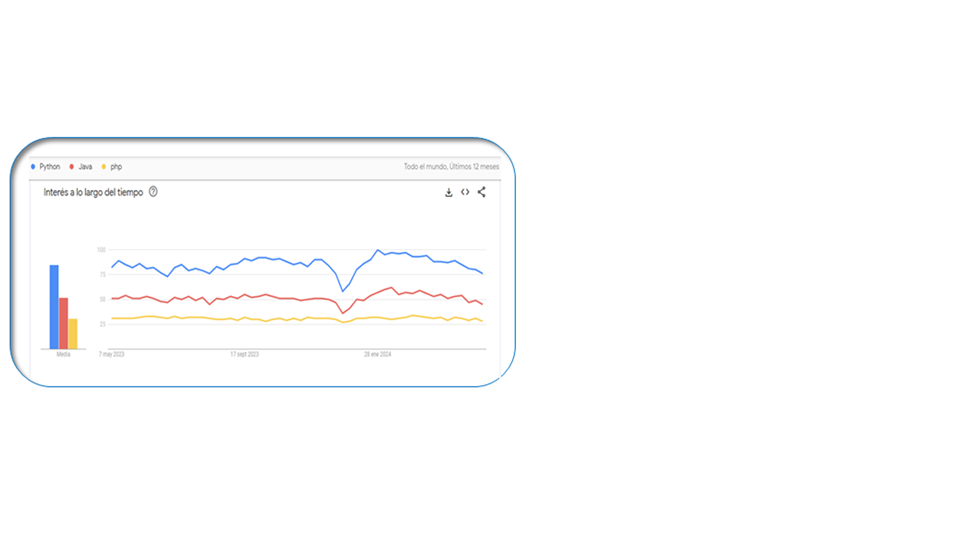
\includegraphics[scale = 1.1]{./images/Google trends.png}
    \caption{Google trends.}
    \label{fig:huella}
    \end{center}
    \end{figure}
En esta tabla, la organización Tiobe nos presenta los lenguajes de programación más buscados en varias plataformas de búsqueda [16]. \\

\subsection{Top 10 de las herramientas mas buscadas en el mundo}

\begin{figure}[H]
    \begin{center}
    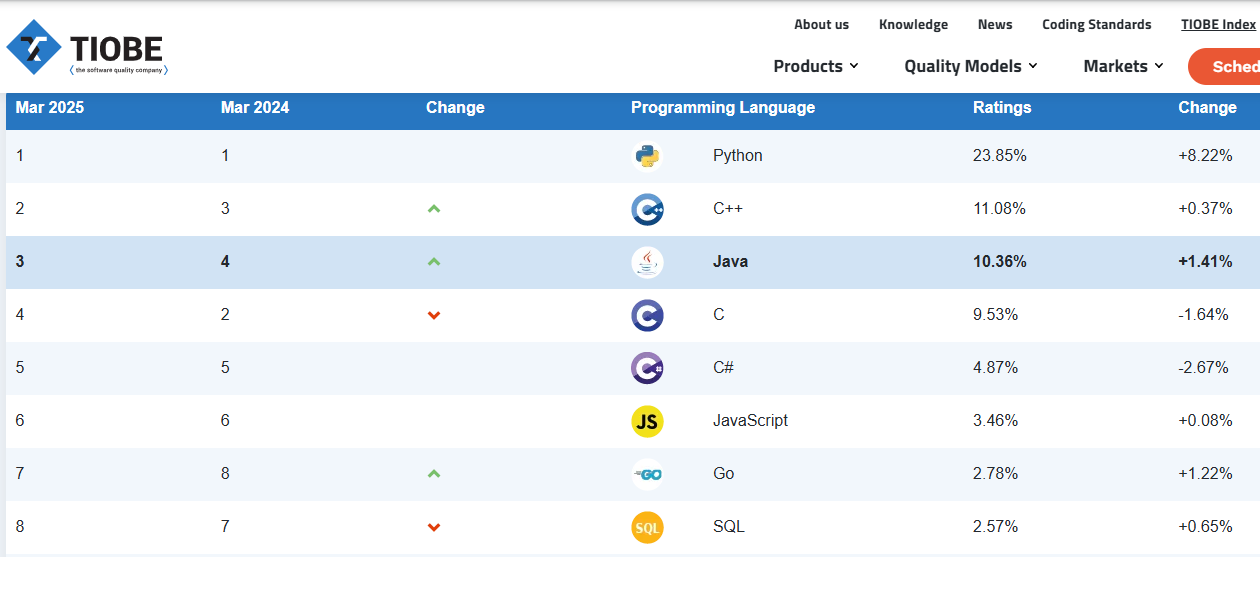
\includegraphics[scale = .4]{./images/tiobe.1.png}
    \caption{Organizacion tiobe.}
    \label{fig:huella}
    \end{center}
    \end{figure}

\subsection{Gráfico de los tres primeros lenguajes en el mundo.} 

Claramente Python está llevando el primer lugar en el último año. \\

\begin{figure}[H]
    \begin{center}
    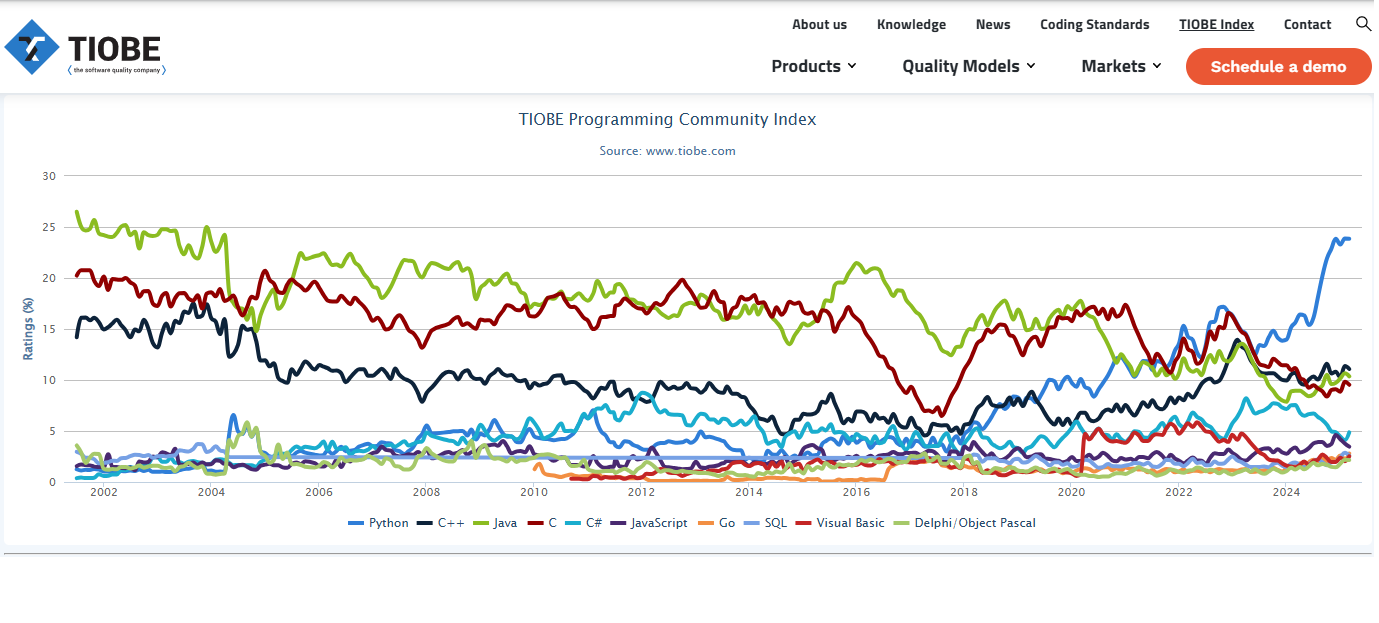
\includegraphics[scale = .4]{./images/tiobe.png}
    \caption{Organizacion tiobe.}
    \label{fig:huella}
    \end{center}
    \end{figure}
\subsection{Características de las herramientas.}

Las características de Python son los siguientes: \\
Python es un lenguaje interpretado, lo que significa que ejecuta directamente el código línea por línea, si existen errores en el código del programa, su ejecución se detiene, así, los programadores pueden encontrar errores en el código con rapidez.
Es un lenguaje fácil de utilizar porque utiliza palabras similares a las del inglés, a diferencia de otros lenguajes de programación, Python no utiliza llaves, en su lugar utiliza sangría. 
Es un lenguaje tipeado dinámicamente, los programadores no tienen que anunciar tipos de variables cuando escriben código porque Python los determina en el tiempo de ejecución. Debido a esto, es posible escribir programas de Python con mayor rapidez.
Es un lenguaje de alto nivel, Python es más cercano a los idiomas humanos que otros lenguajes de programación. Por lo tanto, los programadores no deben preocuparse de sus funcionalidades subyacentes, como la arquitectura y la administración de la memoria.
Es un lenguaje orientado a los objetos, Python considera todo como un objeto, pero también admite otros tipos de programación, como la programación estructurada y la funcional \cite{Bl}. \\

Las características de Java son las siguientes: \\
Es un lenguaje estable, al ser un lenguaje de programación sumamente estable, Java es elegido por las grandes empresas de todo el mundo que desean una tecnología confiable para sus proyectos. Debido a su confiabilidad y credibilidad, las compañías líderes lo incorporan para garantizar que la experiencia de los clientes sea la esperada.
Como lenguaje altamente escalable, Java ofrece capacidades de gestión de tráfico sin rival en ningún otro lenguaje. Esta escalabilidad lo ha convertido en una tecnología fiable para el desarrollo empresarial. Brinda un conjunto de funcionalidades que permite desarrollar aplicaciones web dinámicas e interactivas.
Cuenta con funciones de seguridad integradas que les facilitan a las empresas la protección adecuada de sus datos. Podemos destacar, entre otras características, la autenticación avanzada, los controles de acceso, la encriptación y las inyecciones de SQL. Asimismo, Java tiene funciones para integrar políticas de seguridad, firmas digitales y cifrados.
En Java, existen cientos de bibliotecas que admiten el desarrollo de aplicaciones empresariales. Estas bibliotecas permiten agregar características y funcionalidades de varios tipos, entre las que se incluyen: Google Guava, iText, Protocol Buffers y XStream. Asimismo, hay un amplio conjunto de APIs y herramientas de desarrollo que le facilitan a los desarrolladores añadir funciones que, de otra forma, no serían posibles.
Java funciona muy bien con el ecosistema de Android para crear aplicaciones móviles. Por eso, cada vez son más las empresas que eligen este lenguaje de programación para el desarrollo de aplicaciones Android nativas.
Es la facilidad con la que un software puede ejecutarse sobre diferentes plataformas informáticas, dependiendo lo menos posible de su entorno de ejecución y sin implementar las particularidades de una máquina o sistema concreto. Esto lo logra compilando a código que se ejecuta en una «máquina virtual» de Java. Por ello, puede ejecutarse tanto en entornos Windows como Linux \cite{Tec}. \\

Características de php: \\
Es un código abierto y gratuito. Es un lenguaje orientado a objetos, lo que hace el procesamiento de datos mucho más rápido. 
Permite la separación de códigos, es decir, es posible manipular datos mientras que otros se encuentran estáticos y también es un código limpio y estable. 
Cuenta con una comunidad amplia y activa donde es posible compartir conocimientos y encontrar información. Permite el desarrollo de páginas web complejas y dinámicas. 
Existe una amplia oferta laboral, pues hoy en día son cada vez más las compañías que buscan el desarrollo de sitios web particulares. 
Es un lenguaje que puede ejecutarse en cualquier servidor o sistema operativo siempre y cuando el equipo tenga la capacidad de ejecutar el código sin dificultades por lo tanto es un lenguaje versátil que permite un gran manejo de procesamiento de datos \cite{ph} \\

\subsection{Criterios de evaluación}
Multiplataforma: Se refiere a la capacidad de un lenguaje de programación o software para ejecutarse en múltiples sistemas operativos (Windows, macOS, Linux, etc.) sin necesidad de modificaciones significativas. \\
Software libre: Hace referencia a software que se distribuye con una licencia que permite a los usuarios usarlo, modificarlo y distribuirlo libremente.  \\
Software basado en red: Esto se refiere a aplicaciones o lenguajes de programación diseñados para funcionar o ser ejecutados en un entorno de red, como aplicaciones web o servicios en la nube. \\
Integración de datos: Se refiere a la capacidad del lenguaje o software para conectarse, interactuar y trabajar con diferentes fuentes de datos, como bases de datos SQL, NoSQL, servicios web, etc. \\
Tiempo de implementación: Se refiere al tiempo que se tarda en desarrollar y poner en producción una aplicación o sistema utilizando un lenguaje de programación o software. Esto puede variar según la complejidad del proyecto, la experiencia del desarrollador y las herramientas disponibles. \\
Curva de aprendizaje: Hace referencia a la facilidad con la que los nuevos usuarios pueden aprender a utilizar un lenguaje de programación o software. 

Tablas de comparación \\
\begin{figure}[H]
    \begin{center}
    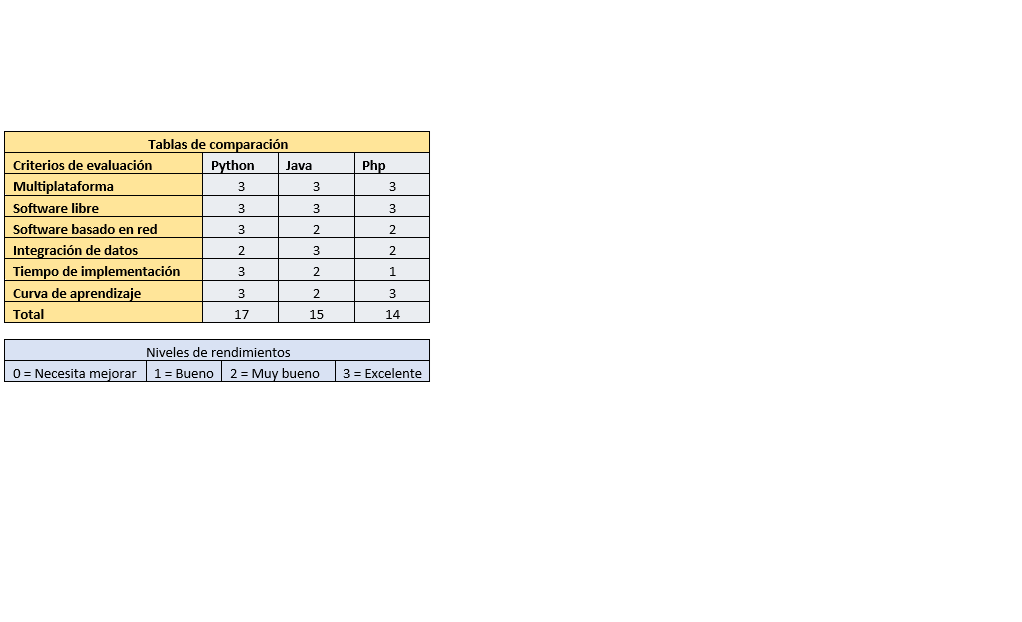
\includegraphics[scale = 1.1]{./images/Tablas de comparacion.png}
    \caption{Tabla de comparacion.}
    \label{fig:huella}
    \end{center}
    \end{figure}

\subsection{Tecnología seleccionada}
Tras analizar diversas opciones, encontramos múltiples herramientas capaces de llevar a cabo el desarrollo de la aplicación requerida. Sin embargo, la elección se basó en criterios clave como la compatibilidad multiplataforma, el corto tiempo de implementación y una curva de aprendizaje más accesible en comparación con otros lenguajes de programación evaluados. \\
En función de estos criterios, la tecnología seleccionada para el desarrollo es Python, debido a su versatilidad, facilidad de uso y amplia comunidad de soporte. \\
Otras tecnologías. \\
Además del lenguaje de programación, el sistema utilizará PostgreSQL como motor de base de datos. PostgreSQL es un sistema gestor de bases de datos relacional, libre y de código abierto, reconocido por su robustez y escalabilidad. Para la administración y gestión de la base de datos, se empleará pgAdmin, una herramienta gráfica que facilita la configuración, monitoreo y mantenimiento del sistema \cite{doc}. \\

\fancyhead{}
\fancyfoot{}
\cfoot{\thepage}

\lhead{Metodos}

\chapter{Metodos}

\section{Introducción }


Este capítulo describe el enfoque metodológico utilizado para desarrollar el Sistema Experto Basado en Reglas para el Monitoreo de Máquinas Críticas. Se detallan los métodos empleados en la recopilación de información, la formulación de reglas y la implementación del sistema. \\
\section{Enfoque}
En este estudio, se adoptó un enfoque cuantitativo basado en reglas para estructurar el conocimiento experto de la fábrica dentro del sistema. \\
Investigación Cuantitativa. \\
Se recopiló y analizó información técnica sobre el estado de las máquinas críticas, considerando parámetros medibles como temperaturas, caudal, y el estado de los compresores y bombas de agua. Esta información permitió definir umbrales de normalidad y anormalidad que fueron incorporados en el sistema experto. \\
\section{Diseño de la Investigación}
Dentro del enfoque cuantitativo, existen dos grandes clasificaciones de diseño de investigación: experimental y no experimental. Para este estudio, se ha adoptado un diseño no experimental, ya que no se manipulan variables de manera controlada, sino que se observan y analizan los estados de las máquinas en su entorno real de operación. \\
Diseño No Experimental \\
En este tipo de diseño, los datos se recopilan sin intervenir en los procesos naturales del sistema. Dentro de esta categoría, la investigación sigue un diseño longitudinal, pues se basa en la recolección continua de datos sobre el estado de las máquinas a lo largo del tiempo. \\

\section{Justificación del Diseño}
El Sistema Experto Basado en Reglas fue desarrollado para analizar información en tiempo real y detectar fallas en las máquinas críticas de la fábrica. Dado que las condiciones operativas varían constantemente, un diseño longitudinal permite evaluar tendencias, detectar anomalías y generar alarmas basadas en patrones históricos. \\
Este enfoque metodológico garantiza que el sistema pueda identificar problemas recurrentes, mejorar la toma de decisiones y mejorar las estrategias de mantenimiento sin necesidad de intervenir artificialmente en los procesos industriales. \\

\section{Fase de Diseño del Sistema Experto}
La fase de diseño fue clave para definir la estructura y los componentes fundamentales del sistema experto de monitoreo. Se llevaron a cabo distintas etapas para garantizar que el sistema fuera modular, eficiente y fácilmente escalable. \\
Diseño de la Arquitectura del Sistema Experto. \\
Se estableció la estructura general del sistema, identificando sus principales módulos y la forma en que interactúan entre sí. La arquitectura definida incluyó los siguientes componentes:

\section{Arquitectura del Sistema.} 

\begin{figure}[H]
    \begin{center}
    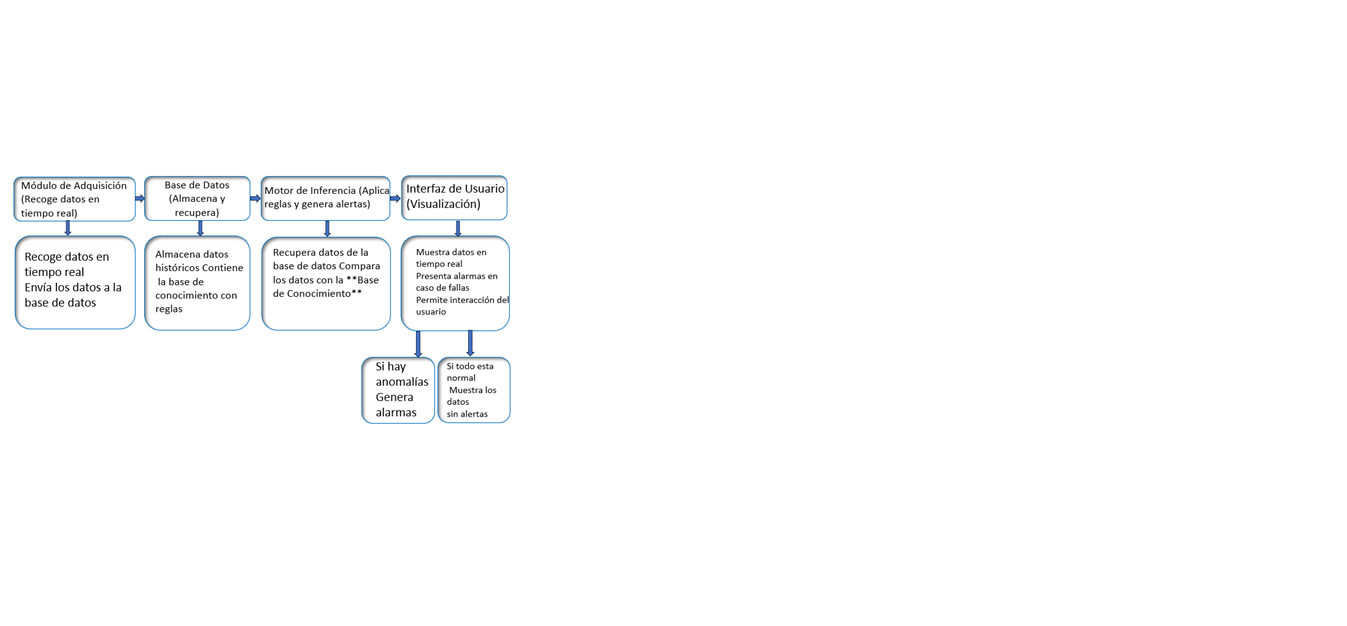
\includegraphics[scale = 1.0]{./images/Arquitectura del sistema experto.png}
    \caption{Arquitectura del sistema.}
    \label{fig:huella}
    \end{center}
    \end{figure}
Módulo de adquisición de datos: \\

Encargado de recibir información en tiempo real desde los sensores instalados en la fábrica. \\
\\
Base de conocimiento basada en reglas: \\
Contiene las reglas que permiten interpretar los datos y determinar el estado del sistema. \\
\\
Motor de inferencia: \\
Responsable de analizar los datos de entrada y aplicar las reglas para generar conclusiones y alertas. \\
\\

Interfaz de usuario:\\
Diseñada para permitir la visualización de datos en tiempo real y la interacción con el usuario. \\
\\
Base de datos:\\

Almacena los datos históricos del sistema y las reglas, asegurando un acceso eficiente. \\
Se definieron las interrelaciones entre estos módulos y el flujo de información que permite su correcto funcionamiento. \\
\\
Diseño de Módulos Funcionales. \\
Para garantizar un desarrollo eficiente y mantenible, el sistema se desglosó en módulos funcionales bien definidos: \\
Módulo de adquisición de datos: Responsable de la captura de datos de los sensores y su transmisión al sistema experto. \\

\begin{figure}[H]
    \begin{center}
    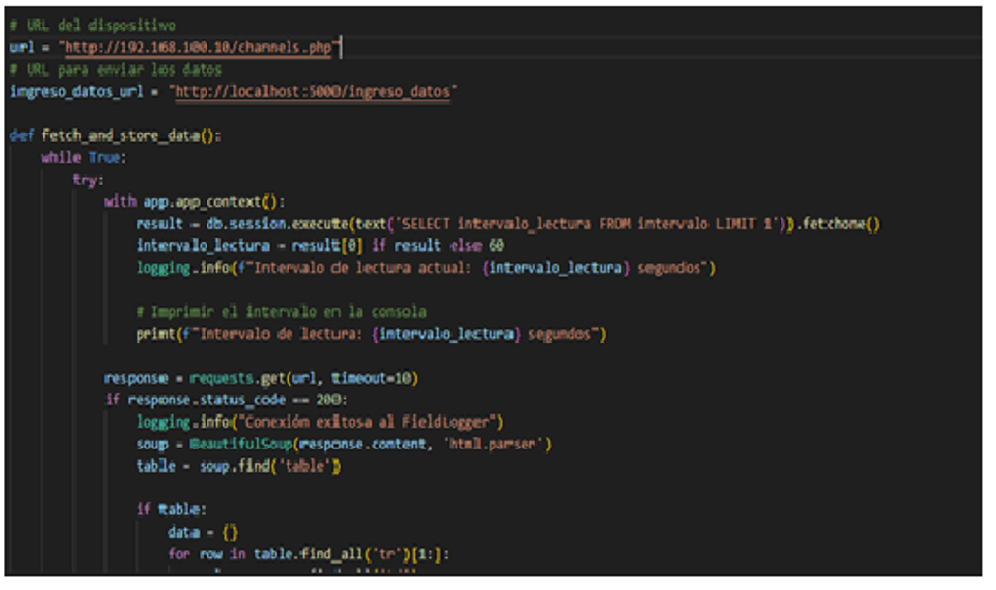
\includegraphics[scale = .5]{./images/Modulo de adquisicion de datos.png}
    \caption{Momdulo de adquisicion de datos.}
    \label{fig:huella}
    \end{center}
    \end{figure}

Módulo de procesamiento de datos: Normaliza y organiza la información para su análisis.\\
Módulo de inferencia: Implementa la lógica de decisión basada en reglas. \\
\\
Módulo de inferencia. \\

\begin{figure}[H]
    \begin{center}
    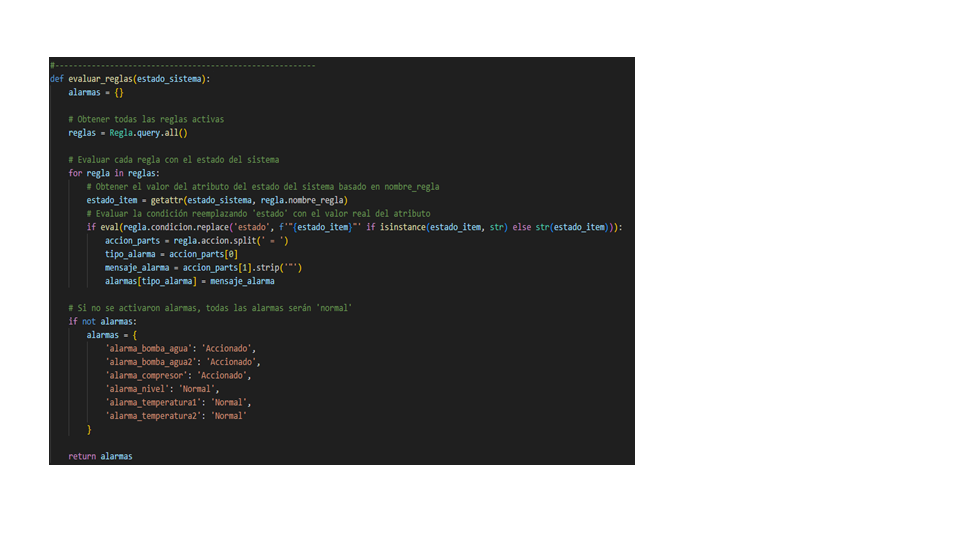
\includegraphics[scale = 0.7]{./images/motor de inferencia.png}
    \caption{Motor de inferencia.}
    \label{fig:huella}
    \end{center}
    \end{figure}


Módulo de visualización: Gestiona la interfaz web y la presentación de datos. \\
Cada módulo se diseñó con interfaces bien definidas para facilitar su integración y escalabilidad. \\

\begin{figure}[H]
    \begin{center}
    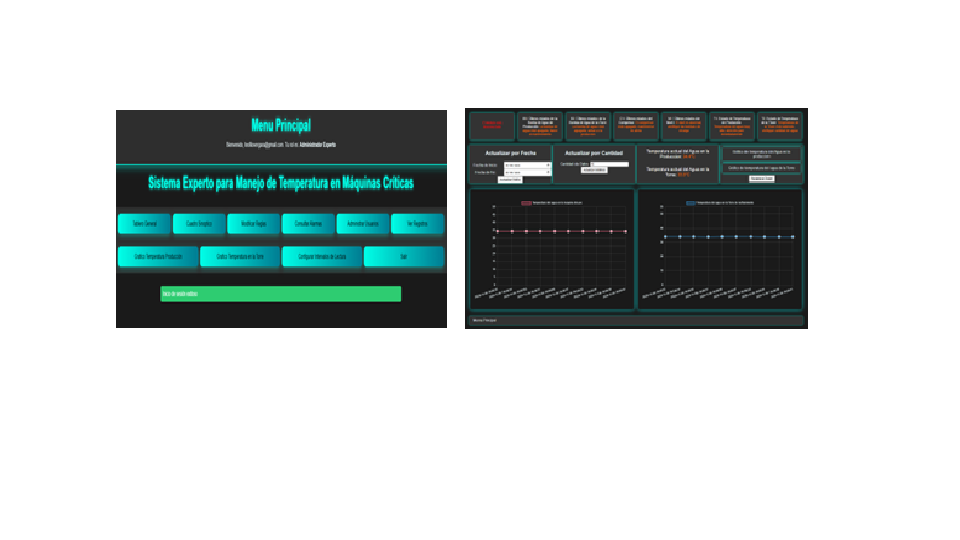
\includegraphics[scale = 0.6]{./images/desarrollo de sistema.png}
    \caption{Base de conocimiento.}
    \label{fig:huella}
    \end{center}
    \end{figure}


Diseño de la Base de Conocimiento \\
La base de conocimiento fue estructurada para facilitar su acceso y mantenimiento. Para ello, se determinaron los siguientes aspectos: \\

\begin{figure}[H]
    \begin{center}
    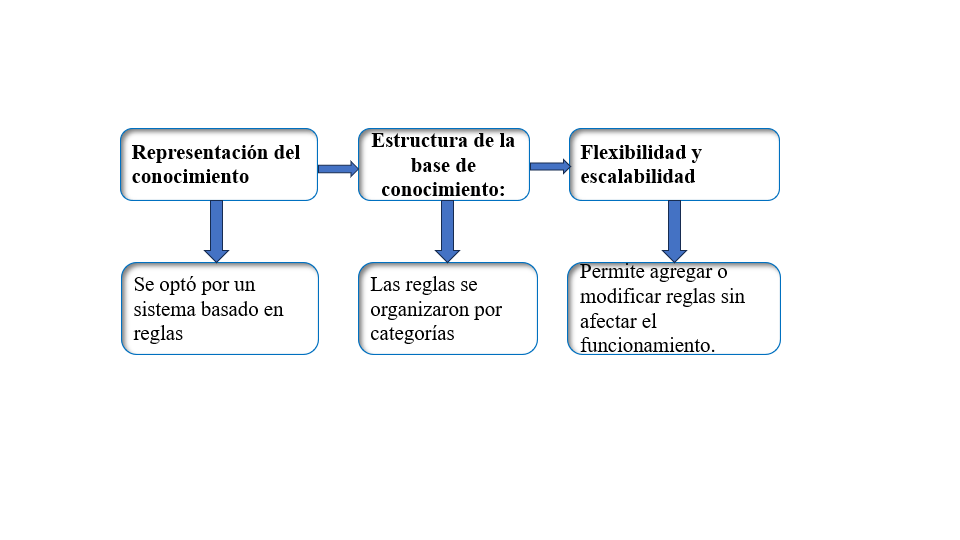
\includegraphics[scale = 0.6]{./images/base de conocimiento.png}
    \caption{Base de conocimiento.}
    \label{fig:huella}
    \end{center}
    \end{figure}

    \subsection{Representación del conocimiento: }
Se optó por un sistema basado en reglas, donde cada regla define un conjunto de condiciones y la acción a tomar en caso de que dichas condiciones se cumplan. \\
Estructura de la base de conocimiento: Las reglas se organizaron por categorías, agrupando aquellas relacionadas con parámetros específicos del sistema (bomba de agua, compresor, caudal, temperatura, etc.).\\
Flexibilidad y escalabilidad: Se diseñó un esquema que permite agregar o modificar reglas sin afectar el funcionamiento general del sistema. \\
\\
Diseño del Motor de Inferencia. 
El motor de inferencia es el encargado de procesar los datos adquiridos y aplicar las reglas de la base de conocimiento para tomar decisiones. \\
Selección del algoritmo de inferencia: Se utilizó un sistema basado en reglas condicionales para evaluar el estado del sistema en función de los datos obtenidos. \\
Optimización del rendimiento: Se definió una estrategia para minimizar el tiempo de respuesta y garantizar el análisis en tiempo real.
Integración con el módulo de adquisición de datos: Se estableció un mecanismo de comunicación eficiente para recibir datos en tiempo real y ejecutar las reglas de inferencia. \\
\\
Diseño de la Interfaz de Usuario\\
Se crearon prototipos de la interfaz web para asegurar una visualización clara y efectiva de la información generada por el sistema. \\
Visualización de datos en tiempo real: Se diseñaron gráficos dinámicos y paneles informativos para mostrar las mediciones del sistema. \\
\\
Gestión de alertas: Se implementó una sección donde el usuario puede ver las alertas generadas por el sistema y su causa. \\
\\

Experiencia de usuario: Se priorizó un diseño intuitivo y accesible, con una paleta de colores con fondo grafito y detalles en naranja oscuro. \\

Funcionamiento del Sistema Experto.\\
El sistema experto está diseñado para facilitar la gestión y monitoreo de los procesos industriales relacionados con los sistemas de refrigeración de agua en la producción de PVC. El sistema está estructurado en base a un esquema de usuarios con diferentes roles, lo que permite una administración eficiente de las funcionalidades según el perfil de cada usuario. \\
Inicio de Sesión (Login) y Roles de Usuario. \\
Al ingresar al sistema, el usuario debe autenticar sus credenciales a través del login. El sistema permite acceder a diferentes secciones dependiendo del rol asignado al usuario. Los roles definidos incluyen: \\
Administrador.\\
Los usuarios con privilegios de Administrador pueden acceder a una sección especial que les permite agregar, editar o eliminar usuarios. Además, pueden asignar o modificar roles a los usuarios, asegurando que las funciones y permisos estén correctamente distribuidos en la organización. Esta funcionalidad garantiza que solo los usuarios adecuados tengan acceso a áreas sensibles del sistema. \\
\\
Administrador experto. \\
Los Administradores expertos tienen la capacidad de modificar las reglas del sistema experto a través de una interfaz dedicada. Estas reglas están relacionadas con el monitoreo de los sistemas críticos de refrigeración. Por ejemplo, un administrador de reglas puede modificar umbrales de temperatura o establecer condiciones de alarma. Esta flexibilidad asegura que el sistema se adapte a diferentes condiciones operativas. \\
Operador: \\
Accede principalmente a las funcionalidades de consulta y visualización, pero con permisos limitados. \\
Cada usuario se verá redirigido a una página principal donde podrá ver las opciones disponibles basadas en su rol. El sistema garantiza que cada usuario solo tenga acceso a las funciones que le corresponden según su perfil. \\
Visualización de Temperaturas.\\
Una de las funcionalidades clave del sistema es la visualización gráfica de las temperaturas de los sistemas de refrigeración. En una página dedicada, se muestra una gráfica en tiempo real con los datos de temperatura recogidos desde el sistema. Los usuarios pueden observar el comportamiento de las temperaturas y detectar posibles desviaciones en el funcionamiento de la maquinaria. Esta página es crucial para los técnicos, ya que les permite identificar rápidamente cualquier irregularidad que pueda afectar el rendimiento del sistema de refrigeración.\\
\\
Cuadro Sinóptico. \\

Otra página importante es el cuadro sinóptico, que proporciona una vista global del estado de todos los sistemas de refrigeración. Esta página se actualiza dinámicamente a partir de los datos almacenados en la base de datos. Los usuarios pueden consultar en tiempo real el estado de cada equipo, incluidas las alarmas activas y las condiciones operativas de los sistemas de refrigeración. Esto permite un monitoreo constante y oportuno, facilitando la detección de fallos y la implementación de acciones correctivas inmediatas.\\

\begin{figure}[H]
\begin{center}
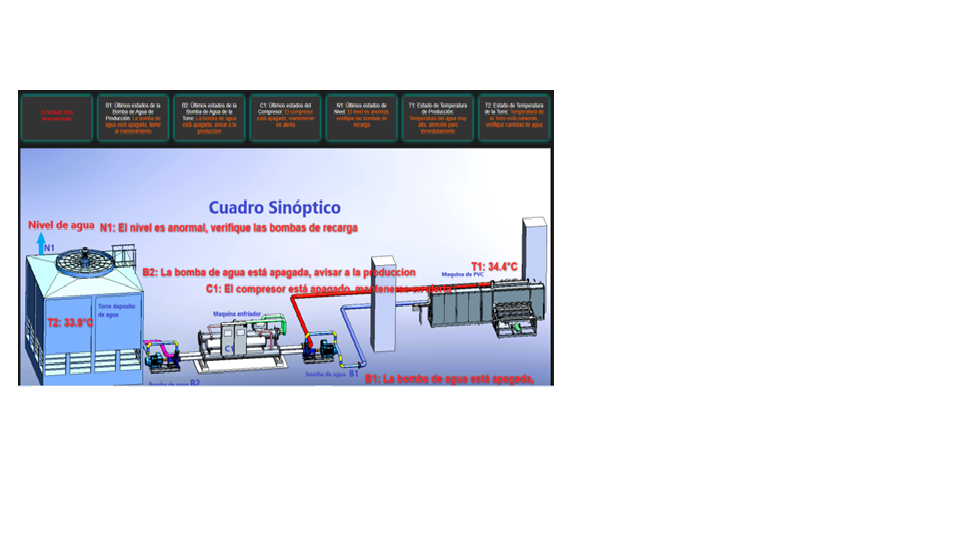
\includegraphics[scale = 0.9]{./images/cuadro sinoptico.png}
\caption{Cuadro sinóptico.}
\label{fig:huella}
\end{center}
\end{figure}

\subsection{Partes principales del código fuente}

\begin{figure}[H]
\begin{center}
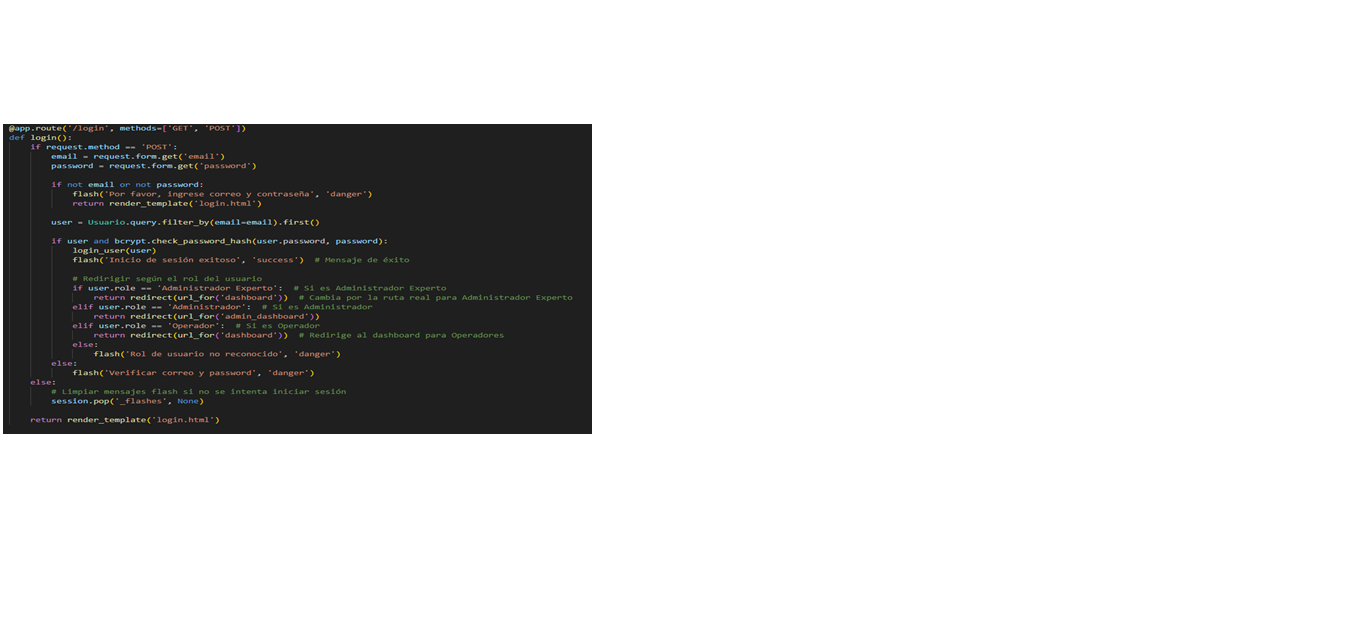
\includegraphics[scale = 0.8]{./images/codigo de login.png}
\caption{Codigo de login.}
\label{fig:huella}
\end{center}
\end{figure}

\begin{figure}[H]
\begin{center}
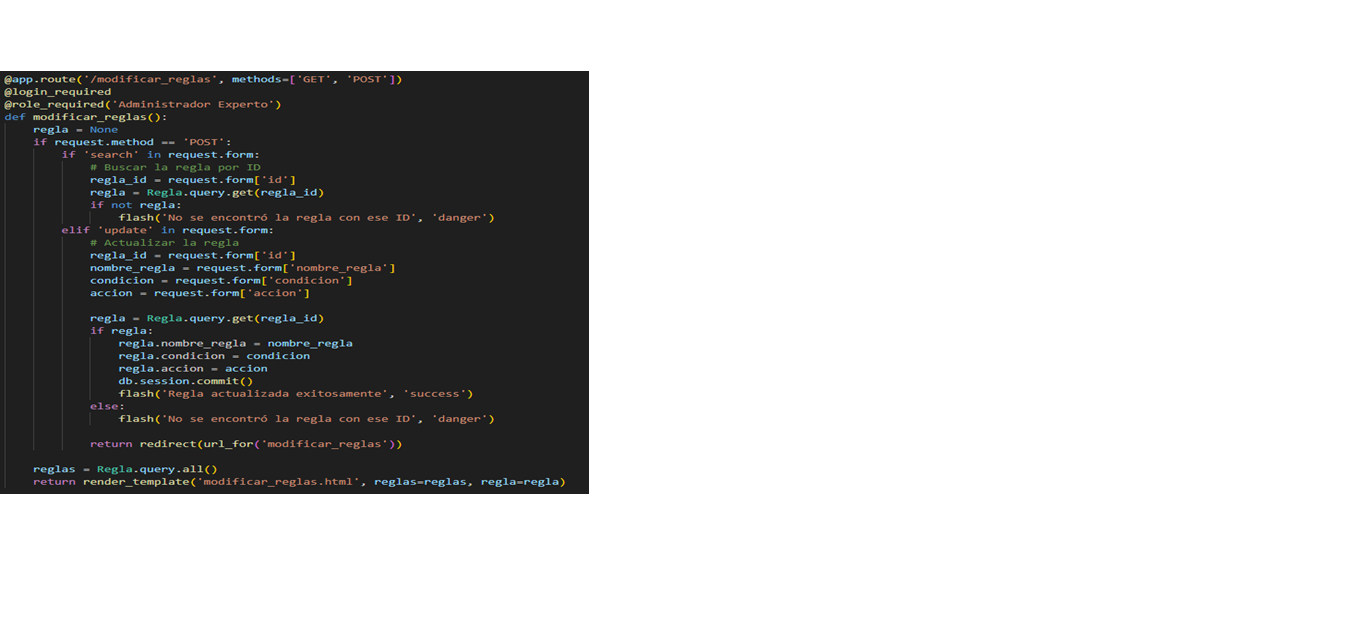
\includegraphics[scale = 0.8]{./images/modificar reglas.png}
 \caption{Codigo para modificar reglas.}
\label{fig:huella}
\end{center}
\end{figure}

\begin{figure}[H]
    \begin{center}
     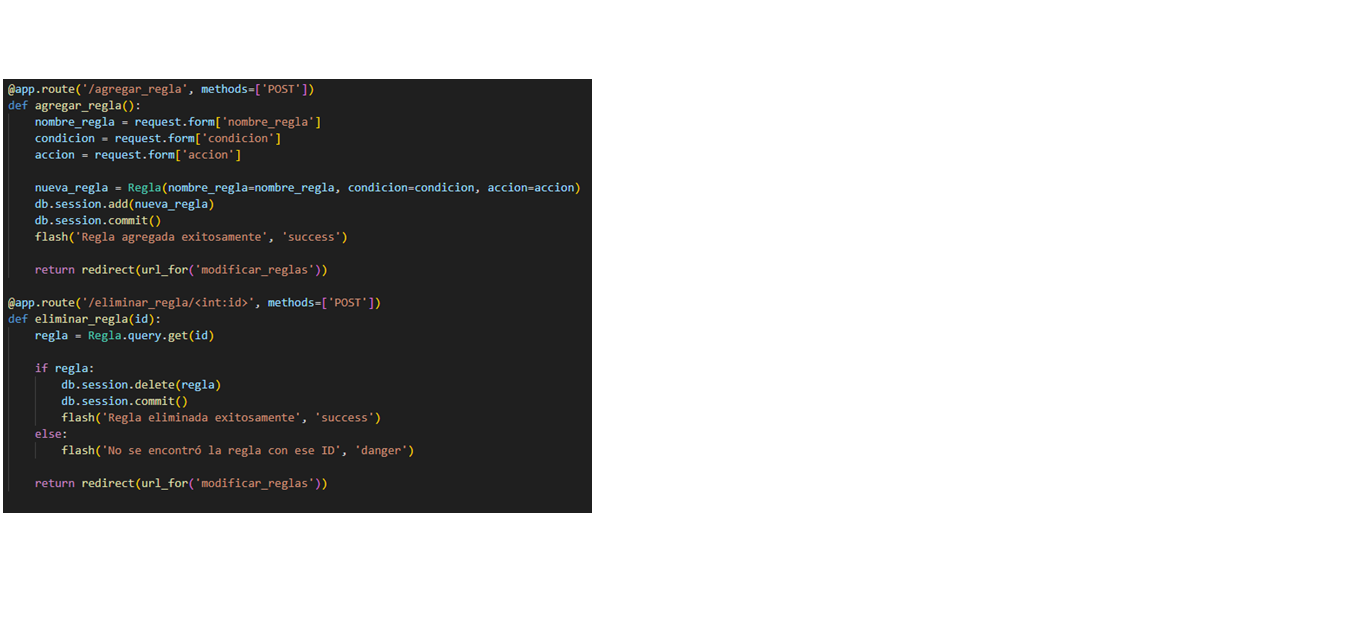
\includegraphics[scale = 0.8]{./images/agregar eliminar.png}
     \caption{Agregar o modificar reglas.}
     \label{fig:huella}
    \end{center}
    \end{figure}

            \begin{figure}[H]
                \begin{center}
                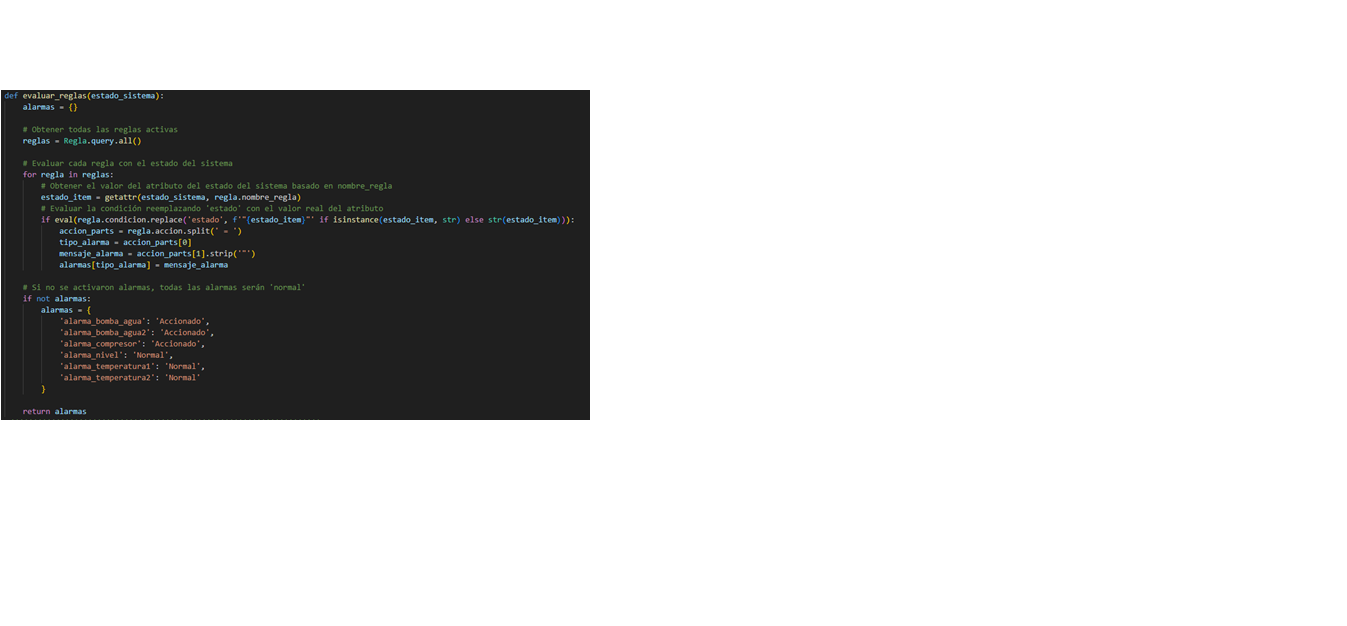
\includegraphics[scale = 0.8]{./images/evaluar reglas.png}
                \caption{Evaluar reglas.}
                \label{fig:huella}
                \end{center}
                \end{figure}
    

\fancyhead{}
\fancyfoot{}
\cfoot{\thepage}

\lhead{Discusión}

\chapter{Discusión}

En este capítulo, que también suele denominarse ``Conclusiones'', se derivan las conclusiones, se explicitan recomendaciones para otros estudios (por ejemplo, sugerir nuevas preguntas, muestras, instrumentos, líneas de investigación, etc.) y se indica lo que sigue y lo que debe hacerse. Se analiza la posibilidad de extender los resultados a una población mayor que la del estudio. Se evalúan las implicaciones, se establece la manera como se respondieron las preguntas de investigación, si se cumplieron o no los objetivos, se relacionan los resultados con los estudios existentes (vincular con el marco teórico y señalar si los resultados coinciden o no con la literatura previa, en qué sí y en qué no). Se reconocen las limitaciones de la investigación, se destaca la importancia y significado de todo el estudio y la forma como encaja en el conocimiento disponible. Se explican los resultados inesperados y cuando no se verificaron las hipótesis es necesario señalar o al menos especular sobre las razones. Recordar que no se deben repetir aquí los resultados sino que se los debe interpretar. La discusión debe redactarse de tal manera que se facilite la toma de decisiones respecto de una teoría, un curso de acción o una problemática. Resumiendo, este capítulo puede ser conceptualmente y dividido en al menos tres secciones, como se ilustra a continuación.

\section{Logros alcanzados}
Descripción de los principales descubrimientos obtenidos como producto de la interpretación de los resultados de la investigación.
\section{Solución del problema de investigación}
Aquí se realiza la discusión propiamente dicha, respondiendo al problema planteado e indicando el nivel de satisfacción de la solución lograda.
\section{Sugerencias para futuras investigaciones}
Todo trabajo de investigación, genera invariablemente como producto colateral, otras interrogantes que suelen ameritar seguir con la investigación. Esto es derivado del caracter abierto, \textit{i.e.}, inacabado, del conocimiento científico. En esta sección se acostumbra hacer referencia a posibles seguimientos de la investigación indicando las interrogantes que conforman nuevos problemas pasibles de ser indagados.   

\backmatter

\cleardoublepage
\addcontentsline{toc}{chapter}{Glosario}
\printglossary
% \printglossaries

\addcontentsline{toc}{chapter}{Anexos}

\cleardoublepage
\fancyhead{}
\fancyfoot{}
\cfoot{\thepage}

\lhead{Anexo A.}
%\rhead{\today}
%\rfoot{\thepage}

\chapter{Anexo A.}
Los apéndices y anexos resultan útiles para describir con mayor profundidad ciertos materiales, sin distraer la lectura del texto principal del reporte o evitar que rompan con el formato de éste. Algunos ejemplos serían el cuestionario utilizado, un código de programa computacional, análisis estadísticos adicionales, la demostración matemática de un teorema complicado, fotografías testimoniales, etc.



\cleardoublepage
\addcontentsline{toc}{chapter}{Referencias bibliogr\'aficas}

\bibliographystyle{IEEEtran-castellano}
\bibliography{test}

\end{document}

